\documentclass{standalone}
\begin{document}
This interpretation, that the Stabiliser Rank of a resource state allows us to quantify in some sense its computational power, naturally leads to the question of how the Stabiliser rank scales for alternative resources. \\
Here, we consider single qubit resource states $\ket{R}$, which we use in conjunction with Clifford group operations. The state $\ket{R}$ is an eigenstate of an operator $R\in\mathcal{C}_{n}$, and can be generated by applying a Unitary $U$ to a stabiliser state. We can then show that
\begin{align}
\begin{split}
R\ket{R} &= R U\ket{\phi} : \exists \mathcal{S}_{\phi} \\
U^{\dagger}\ket{R} &= U^{\dagger}U\ket{\phi} = \ket{\phi}\\
\implies UsU^{\dagger} &= R \forall s\in\mathcal{S}_{\phi}\\
&\implies U \in\mathcal{C}_{n+1} \\
\end{split}
\end{align}
As an example, the edge-type magic state $\ket{H}$ is so named as it is an eigenstate of the Hadamard operator $H\in\mathcal{C}_{2}$, and thus the state is generated by a transform $U\in\mathcal{C}_{3}$, and allows us to realise this operation $U$.
\par
In the first section, we will examine Conjecture~\ref{thm:magicrank} made by Bravyi, Smolin \& Smith, by extending their method to find the asymptotic behaviour of $\chi(\ket{F^{\otimes t}})$. \\
We will then use a pair of computational methods, a brute-force search and a proposed resource measure `Robustness', to try and find explicit values of $\chi$ for arbitrary states, magic states, and finally for resrouce states that would allow us to realise gates from higher levels in the Clifford Hierarchy.

\section{Stabiliser Rank of the Face States}\label{sec:frank}
The face states are a family of $8$ Clifford-equivalent magic states with a Bloch vector that projects out from the faces on the `simulable' octohedron shown in Fig.~\ref{fig:octohedron}. We will focus on the state $\ket{F}$, which has a description in the computational basis~\cite{Bravyi2005}
\begin{equation}\label{eq:Fstate}
\ket{F} = \cos(\beta)\ket{0}+\mathe^{i\frac{\pi}{4}}\sin(\beta)\ket{1}\;:\;2\beta = \cos^{-1}(\frac{1}{\sqrt{3}}).
\end{equation}
This state is also called $\ket{T}$ in the original paper on magic state distillation~\cite{Bravyi2005}, and $\ket{R}$ by bravyi, Smoilin \& Smith~\cite{Bravyi2015}.
\par
This state is an eigenstate of an operator we shall refer to as $\Delta$, as it is a rotation of the triangular $F$-state face in the octohedron around the axis $\ket{F}$. In particular, it rotates between the states that form the corners of the face.
\begin{align}
\begin{split}
    \Delta\ket{0} &= \ket{+i}\\
    \Delta\ket{+i} &= \ket{+} \\
    \Delta{\ket{+}} &= \ket{0} \\
\end{split}
\end{align}
Because this operator maps stabiliser states to stabiliser states, we can see that it is a Clifford group operation, and thus $\ket{F}$ allows us to realise an operation $U_{F}\in\mathcal{C}_{3}$.
\par
To apply the results of Bravyi \& Gosset discussion in Section~\ref{sec:edgebound}, we need to find a similar expression in terms of $t$-bit strings. As the state is a symmetric point between three stabiliser states, we can define a ternary basis
\begin{align}
\begin{split}
\ket{\tilde{0}} &= \ket{0}\\
\ket{\tilde{1}} &= \ket{+i}\\
\ket{\tilde{2}} &= \ket{+}\\
\end{split}
\end{align}
which has the desired property that each state has the same overlap with $\ket{F}$
\begin{equation}
\left|\braket{\tilde{x}}{F}\right|^{2} = \cos^{2}(\beta)\equiv\mu^{2}.
\end{equation}
\par
Including the relevant phase corrections, we can thus write $t$ copies of the $F$ state as a sum over $t$-bit ternary strings
\begin{equation}
    \ket{F^{\otimes t}} = \frac{1}{(3\mu)^{t}}\sum_{x\in\mathbb{F}_{3}^{t}}\mathe^{i(\vert x\vert_{2}-\vert x\vert_{1})\phi}\ket{\tilde{x}_{1}\otimes\cdots\otimes\tilde{x}_{t}}
\end{equation}
where the angle $\phi$ is equal to $\frac{\pi}{12}$, and $\vert x\vert_{1,2}$ is the $1$ and $2$-weight of the string $x$.\\
This decomposition, however, contains $3^{t}$ stabiliser states, and so is actually overcomplete compared to the computational basis representation. 
\par
We thus need a way to define a normalised state associated to linear subpspaces $\mathcal{L}\subseteq\mathbb{F}_{3}^{t}$, such that we can find decompositions with $\chi=3^{k}$. This requires redefining the partition function $Z_{F}(\mathcal{L})=\sum_{x\in\mathcal{L}}f(x)$.\\
The additional complication here is the presence of a complex phase in the state. Again, the amplitude of the overlap between the three states is equal
\[\vert\braket{\tilde{x}}{\tilde{y}}\vert = 2^{-\frac{(1-\delta_{xy})}{2}},\]
where $\delta_{xy}$ is the Kronecker delta, but we also have that 
\[
\braket{\tilde{1}}{\tilde{2}}=\frac{1}{\sqrt{2}} 
\mathe^{-i\frac{\pi}{4}} 
= (\braket{\tilde{2}}{\tilde{1}})^*
\]
Thus, the absolute value of the overlap between a pair of strings will have a magnitude given by the difference in their Hamming weights, and an additional correction given by the phases, giving
\begin{equation}
    f(x)\equiv 2^{-\frac{\vert x\vert}{2}}\cos((\vert x\vert_{2}-\vert x\vert_{1})\phi).
\end{equation}
This was verified numerically by calculating the overlap between different linear subspaces. Thus, we can define the appropriate normalised state
\begin{equation}
    \ket{\mathcal{L}}=\frac{1}{\sqrt{3^{k}Z_{F}(\mathcal{L})}}\sum_{x\in\mathcal{L}}
    \mathe^{i(\vert x\vert_{2}-\vert x\vert_{1})\phi}\ket{\tilde{x}_{1}\otimes\cdots\otimes\tilde{x}_{t}}
\end{equation}
\par
Once we have this explicit form for the stabiliser states, we can thus verify a similar form for the overlap between the magic states and a linear subspace
\begin{equation}\label{eq:foverlap}
\vert\braket{F^{\otimes t}}{\mathcal{L}}\vert^{2}=\frac{3^{k}\mu^{2t}}{Z_{F}(\mathcal{L})}.
\end{equation}
which arises from the fact that each bit in each string has overlap $\mu$ with the state $\ket{F}$, and that there are $3^{k}$ such strings, giving 
\[\left|\braket{F^{\otimes t}}{\mathcal{L}}\right|^{2}=\left(\frac{3^{k}\mu^{t}}{\sqrt{3^{k}Z_{F}(\mathcal{L})}}\right)^{2}=\frac{3^{k}\mu^{2t}}{Z_{F}(\mathcal{L})}.\]
\par
We can use this result to prove an equivalent of Lemma~\ref{thm:expectation}. In particular, we need to evaulute the expression
\[\sum_{x\in\mathbb{F}_{3}^{t}\setminus 0^{t}}f(x)\mathbb{E}(\chi_{\mathcal{L}}(x))\] 
The partition function for the string $\ket{\tilde{0}^{\otimes t}}$ is $1$. We can use the fact that $\left|\braket{F^{\otimes t}}{\mathbb{F}_{3}^{t}}\right|^{2}=1$, and rearrange Eq.~\ref{eq:foverlap} to express it in terms of $Z_{F}(\mathcal{L})$, to give
\begin{align}
\begin{split}
\sum_{x\in\mathbb{F}_{3}^{t}\setminus 0^{t}}f(x) &= 
\frac{3^{t}\mu^{2t}}{\left|\braket{F^{\otimes t}}{\mathbb{F}_{3}^{t}}\right|^{2}} - 1\\
&= 3^{t}\mu^{2t}-1
\end{split}
\end{align}
We also note that, as the indicator function $\chi_{\mathcal{L}}(x)$ is 1 if and only if $x\in\mathcal{L}$, and as $\chi_{\mathcal{L}}(0^{t})=1\forall\mathcal{L}$ as the zero-string is the `identity' element for these subspaces, it's expectation value is simply given by
\begin{equation}
\mathbb{E}\left(\chi_{\mathcal{L}}(x)\right)=\frac{3^{t}-1}{3^{k}-1}
\end{equation}
the relative number of elements in the subspace. 
\par
Thus, we can prove that Lemma~\ref{thm:expectation} translates to these linear subspaces on $\mathbb{F}_{3}^{t}$, namely
\begin{equation}
\mathbb{E}\left( Z_{F}(\mathcal{L}) \right)\leq 1+3^{k}\mu^{2t}.
\end{equation}
\par
The subsequent argument given in Eq.~\ref{eq:markovineq}, using Markov's inequality to show that we can find $\mathcal{L}^{\star}:Z\left(\mathcal{L}^{\star}\right)\leq(1+2^{k}\nu^{2t})\left(1+\frac{\delta}{2}\right)$, seems to apply directly for $Z_{f}$ and the linear subspaces on $\mathbb{F}_{3}^{t}$, provided we fix
\begin{align}
\label{eq:fix3k}
9\geq 3^{k}\mu^{2t}\delta\geq 3\\
\label{eq:Zfbound}
\implies\exists\;\mathcal{L}^{\star} : Z_{f}\left(\mathcal{L}^{\star}\right)\leq \left(1+3^{k}\mu^{2t}\right)\left(1+\frac{\delta}{2}\right).
\end{align}
Thus, we can use this inequality on $Z_{f}(\mathcal{L})$ in Eq.~\ref{eq:foverlap}, to show that this state will $\delta$ approximate $\ket{F^{\otimes t}}$.
\begin{align}
\begin{split}
    \left| \braket{F^{\otimes t}}{\mathcal{L}^{\star}}\right|^{2} &\geq
    \frac{3^{k}\mu^{2t}}{\left(1+3^{k}\mu^{2t}\right)\left(1+\frac{\delta}{2}\right)}  \\
    &\geq \frac{1}{\left(1+3^{-k}\mu^{-2t}\right)\left(1+\frac{\delta}{2}\right)}\\
    &\geq \frac{1}{\left(1+\frac{\delta}{2}\right)^{2}} \qquad \text{\small{From Eq.~\ref{eq:fix3k}}}\\
    &\geq 1-\delta \\
\end{split}
\end{align}
This resulting state has a stabiliser rank 
\begin{equation}
\chi=3^{k}\leq 9\mu^{-2t}\delta^{-1} = O\left(\mu^{-2t}\delta^{-1}\right)=O\left(2^{\gamma_{F}t}\delta^{-1}\right)
\end{equation}
where the scaling factor $\gamma_{F}$ is obtained by using the properties of the logarithm to rewrite $\mu^{-2t}=2^{-2t\log_{2}(\mu)}$, giving $\gamma_{F}\approx0.345$.\\
Lemma~\ref{thm:scalinglemma} then follows immediately for the face-type magic states, as it only depends on the maximal value of the overlap between a stabiliser state and the magic state. In this case, it is given by $\mu=\cos(\beta)$, and gives the bound $\chi=\Omega\left(\mu^{-2t}=2^{\gamma_{F}t}\right)$.
\par
Thus, by defining these approximate decompositions in to ternary strings, we have been able to show that the stabiliser rank of a face-type state has a larger asymptotic bound that for edge-type states. Additionally, if Conjecture~\ref{thm:minscaling} holds, which seems evident from the proof of Lemma~\ref{thm:scalinglemma}, then these states have a stabiliser rank which is strictly larger than for the edge-type states.

\section{Explicit Stabiliser Rank Decomposition}\label{sec:decompositions}
The technique used above to bound the stabiliser rank of a given state does not easily generalise, because it requires that the state be decomposable into a symmetric superposition of stabliser states. This is satisfied by magic states, due to their definition as symmetric points between the single-qubit stabiliser states, but doesn't apply for more general resource states. \\
In particular, we would like to analyse the stabiliser rank for resource states that can be used to realise gates from higher levels in the Clifford hierarchy. An easy way to generate such states is to make use of an observation about the Pauli $Z$ operator. By definition as a Pauli operator, $Z$ is in level $\mathcal{C}_{1}$. It's squre-root, the Phase gate, is a Clifford operation, and thus $\in\mathcal{C}_{2}$. The root of the phase gate, $T$, is another level higher, $\in\mathcal{C}_{3}$. This seems to suggest that taking repeated roots of the gate $Z$ generators operators from successuvely higher levels of the Clifford hierarchy. This is indeed the case.
% , which can be verified from the action of these gates on generators of the Pauli group, $X$ and $Z$.
% \par
% The general form of the $n$-th root of a $Z$ gate is
% \begin{equation}
%     Z^{-\frac{1}{n}} = \begin{pmatrix} 1 & 0 \\ 0 & \mathe^{\frac{\mathi\pi}{(n)}} \\ \end{pmatrix} 
% \end{equation}
% which is equal to a pahse gate with angle $\frac{\pi}{n}$, denoted $R_{\frac{\pi}{n}}$. For a Pauli $X$, such a gate acts as 
% \begin{equation}
%     R_{\phi}XR^{\dagger}_{\phi} = \begin{pmatrix}0 & \mathe^{-\mathi\phi} \\ \mathe^{\mathi\phi} & 0 \\ \end{pmatrix}
% \end{equation}
% which is not a Pauli operator for $\phi\notin\{0,\frac{\pi}{2},\pi,\frac{3\pi}{2}$. 
\par
These operators are diagonal and live in $\mathcal{C}_{n\geq3}$, and thus they meet the criteria to be realised using the state injection method discussed in Section~\ref{sec:msi}. This means the corresponding resource state can be generating by acting the operator $Z^{\frac{1}{n}}:n\;\text{mod } 2=0$ on the state $\ket{+}$. \\
However, as these states are given by a rotation of the state $\ket{+}$ by an angle $\phi<\frac{\pi}{2}$ along the equator of the Bloch sphere, they are not symmetric points between pairs of stabiliser states. This means we will need to determine their stabiliser rank explicitly. 
\par
As discussed in Section~\ref{sec:srank}, Brayi, Smolin \& Smith found approximate values for the stabiliser rank of $\ket{H}$ for up to $6$ qubits. They did this by implementing a random-walk within the space of $n$-qubit stabiliser states, seeking to find a decomposition set $\tilde{\phi}:\norm{\Pi_{\tilde{\phi}}\ket{H^{\otimes n}}}=1$~\cite{Bravyi2015}. \par
\begin{algorithm}[!h]
\caption{Random Walk on Stabiliser States}
\begin{algorithmic}[1]
\Require $\beta_{init},\beta_{max},M,$ target integer $\chi$
\State $\tilde{\phi} \leftarrow \left(\phi_{1},\cdots\phi_{\chi}\right)$ where each $\phi_{a}$ is chosen at random.
\State $\beta \leftarrow \beta_{init}$
\While{$\beta < \beta_{max}$}
    \For{$i=0$ to $100$}
        \State Evaulate $F(\tilde{\phi})=\norm{\Pi_{\phi}\ket{H^{\otimes n}}}$
        \If{$F(\tilde{\phi})=1$}
            \State \Return $\tilde{\phi}$
        \EndIf
        \State Pick random integer $a$ and random Pauli $P\in\mathcal{P}_{n}$
        \State $\phi_{a}'\leftarrow c\left(\mathbb{I}+P\right)\phi_{a}$
        \State $\tilde{\phi}' \leftarrow (\phi_{1},\cdots,\phi'_{a},\cdots\phi_{\chi})$
        \If{$F(\tilde{\phi}')>F(\tilde{\phi})$}
            \State $\tilde{\phi}\leftarrow\tilde{\phi}'$
        \Else
            \State $p_{accept}\leftarrow \exp[-\beta(F(\tilde{\phi})-F(\tilde{\phi}')]$
            \State Pick random $r\in [0,1]$
            \If{$r>p_{accept}$}
                \State $\tilde{\phi}\leftarrow\tilde{\phi}'$
            \EndIf
        \EndIf
    \EndFor
    \State $\beta\leftarrow \beta + \left( \frac{\beta_{max}-\beta_{init}}{M} \right)$
\EndWhile
\State \Return No decomposition found.
\end{algorithmic}
\end{algorithm}
In this algorithm, $\beta$ is a positive-valued parameter analagous to an inverse temperature. This algorithm then resembles a form of Simulated annealing, where we `walk' througb an energy landscape defined by the objective function $F$ trying to find a global minimum, and move `up' the energy landscape with a probability given by the Boltzmann distribution for $\beta$.
\par
However, we would like to find minimal decompositions deterministically for a small number of qubits to be able to state categorically the relative Stabiliser Rank of different resource states. We attempt this using two methods: Brute-Force Search, and a resource measure called Robustness.
\subsection{Computationally Generating Stabiliser States}
Both techniques require us to computationally generate the stabiliser states on $n$ qubits. The number of such states grows rapidly in the number of qubits, and is equal to~\cite{Aaronson2004a}
\begin{equation}\label{eq:nstabs}
    N_{\phi}=2^{n}\prod_{k=0}^{n-1}\left(2^{n-k}+1\right).
\end{equation}
To find the states, we must first build all $n$-qubit stabiliser groups, which we can do by finding their sets of $n$ generators. For each group $\mathcal{S}=\langle s_{1},\cdots,s_{n}\rangle$, we can then build a projector on to the stabiliser space~\cite{Gottesman1997}
\begin{equation}\label{eq:stabproj}
    \Pi_{\mathcal{S}} = \prod_{i=1}^{n} \frac{1}{2}\left(\mathbb{I}+s_{i}\right)
\end{equation}
and the corresponding state can be found by finding it's $+1$ eigenstate.
\par
To generate the stabiliser groups, we employed the binary string representation used by Aaronson\& Gottesman, which was described in Section~\ref{sec:CHP}. Namely, a Pauli operator is defined by $2n+1$ bits: $x_{i}:i\in\{1,\cdots,n\}$, $z_{i}:i\in\{1,\cdots,n\}$ and $r$. The global phase is given by $-1^{r}$, and the $i$th operator in the tensor product by the bits $x_{i},z_{i}$. \\
This allows us to efficiently generate all $n$-qubit Pauli operators with real-valued phase by generating the binary strings $B$ for the numbers $0$ to $2^{2n+1}-1$~\cite{Aaronson2004a}.\\
\par
We can try to generate a stabiliser group by picking a set of $n$ strings from this full set, and generating the corresponding linear subspace by combining the strings under binary addition. To be a valid stabiliser state, we must first check that all $n$ strings mutually commute. We note that two $n$-qubit Pauli operators commute if an even number of qubits are acted on by a pair of Pauli operators. Otherwise, the operators anticommute. For example, 
\begin{align*}
\comm{X\otimes\mathbb{I}\otimes X}{Z\otimes\mathbb{I}\otimes Z}= 0\\
\acomm{X\otimes X\otimes X}{Z\otimes Z\otimes Z} = 0. \\
\end{align*}
In this binary representation, the commutivity of two pauli operators represnted by strings $B_{h},B_{i}$ can be efficiently checked by evaluating their symplectic inner product
\begin{equation}\label{eq:sympprod}
    B_{h}\cdot B_{i} \equiv x_{h,1}z_{i,1}\oplus\cdots\oplus x_{h,n}z_{i,n}\oplus z_{h,1}x_{i,1}\oplus\cdots\oplus z_{h,n}x_{i,n}
\end{equation}
where the addition is modulo 2. The corresponding Pauli operators commute if their binary representations have a symplectic inner product of $0$, and anticommute otherwise.\\
To describe a stabiliser space, the subspace then generated by these commuting operators must contain $2^{n}$ elements, which can be used as a way to check candidate spaces. The resulting space also cannot contain the string corresponding to $0\cdots01$, as this element is equivalent to $-1\mathbb{I}$. Any Pauli subgroup containing the element $-1\mathbb{I}$ cannot have be a stabiliser group, as $-\mathbb{I}\ket{\psi}=-\ket{\psi}$. \\
If the resulting group hadn't previously been found, it was then stored. Otherwise, the candidate group was discarded.
\par
In practice, this method found more `unique' stabiliser groups than expected from Eq.~\ref{eq:nstabs}. This was because the technique was identifying as distinct two groups equivalent up to global phase. Instead, we noted that there are $2^{n}$ ways of distributing the phase between the $n$ generators. For example, on two qubits
\begin{align*}
    \mathcal{S}&=\langle s_{1},s_{2}\rangle \\
    &\neq \langle -s_{1},s_{2}\rangle \\
    &\neq \langle s_{1},-s_{2}\rangle \\
    &\neq \langle -s_{1},-s_{2}\rangle. \\
\end{align*}
Thus, we can generate the full set of stabiliser groups but first generating the $\frac{N_{\phi}}{2^{n}}$ groups with all-positive Pauli operators, and then adding phase to the resulting generators `by hand'. This full method is outlined in Algorithm~\ref{alg:gengroups}, and was implemented in Python using \texttt{Qutip}~\cite{Johansson2012} and the \href{https://github.com/ilanschnell/bitarray}{\texttt{bitarray}} library.
\begin{algorithm}
\caption{Generating $n$ qubit stabiliser groups}
\label{alg:gengroups}
\begin{algorithmic}
\Function{StringsToPauli}{$G$}
    \State $\mathcal{S}\leftarrow\emptyset$
    \For{$g\in G$}
        \State $\mathcal{S}\leftarrow\mathcal{S}\cup \bigotimes_{i=1}^{n} i^{x_{i}\wedge z_{i}}X^{x_{i}}Z^{z_{i}}$ \Comment{where $g = (x_{1}z_{1}\cdots x_{n}z_{n})\in\mathbb{F}_{2}^{2n}$}
    \EndFor
    \State \Return $\mathcal{S}$
\EndFunction
\end{algorithmic}
\begin{algorithmic}[1]
\Require $n$ \Comment{Number of qubits}
\Require \Call{GetEigenstate}{Projector}
\State S $\leftarrow \mathbb{F}_{2}^{n}$, Generators $\leftarrow \emptyset$, States $\leftarrow\emptyset$
\State TotalGenerators $\leftarrow \frac{N_{\phi}}{2^{n}}$ \Comment{where $N_{\phi}$ is defined in Eq.~\ref{eq:nstabs}.}
\While{$|$Generators$|$ < TotalGenerators}
    \State $G = \{g_{1},\cdots,g_{n}\}\subseteq S$
    \If{$\comm{g_{i}}{g_{j}}=0\;\forall\;g_{i},g_{j}\in G$}
        \State $\mathcal{L}\leftarrow \langle g_{1},\cdots,g_{n}\rangle$
        \If{$-\mathbb{I}\in\mathcal{L}$ \textbf{or} $\left|\mathcal{L}\right| \neq 2^{n}$}
            \State Reject candidate
        \EndIf
        \If{$\mathcal{L}\notin$ Generators}
            \State Generators$\leftarrow$ Generators $\cup \{\mathcal{L}\}$
        \EndIf
    \EndIf
\EndWhile
\For{$G\in$ Generators}
    \State $\mathcal{S}$ = \Call{StringsToPauli}{G}
    \State Projector $\leftarrow \prod_{i=1}^{n}\frac{1}{2}\left(\mathbb{I} + s_{i}\right)\quad \forall s_{i}:\mathcal{S}=\langle s_{1},\cdots,s_{n}\rangle$
    \State States $\leftarrow$ states $\cup $ \Call{GetEigenstate}{Projector}
    \For{$\tilde{x}\in\mathbb{F}_{2}^{n}\setminus 0^{n}$}
        \State Projector $\leftarrow \prod_{i=1}^{n}\frac{1}{2}\left(\mathbb{I} + -1^{\tilde{x}_{i}}s_{i}\right)\quad \forall s_{i}:\mathcal{S}=\langle s_{1},\cdots,s_{n}\rangle$
        \State States $\leftarrow$ states $\cup $ \Call{GetEigenstate}{Projector}
    \EndFor
\EndFor
\State \Return States
\end{algorithmic}
\end{algorithm}
\subsection{Brute Force Search}
This is the simplst method of finding a decomposition in to magic states. For a given $n$, we pick a set of $i$ states from the set of all $n$-quit stabiliser states. We then have to build the projector on to the space generated by these states, and test the overlap with the target states $\ket{R^{\otimes n}}$. If it is equal to one, we are done. Else, we continue testing all $i$ states. If this is exhausted, we increment $i$ and resume. This will continue up to $i=2^{n}$, where the method will find the computational basis decomposition and exit. Pseudocode for the method is given in Algorithm~\ref{alg:brutef}.
\par
The projector onto the space spanned by the Stabiliser states is found using Gram-Schmidt orthoganlisation~\cite{Nielsen2000}. This well established technique for building an orthogonal basis for the space spanned by a collection of vectors $\{u\}$. As the Stabiliser states are known to form a mutually unbised basis~\cite{Howard2013}, this condition is always met for combinations of Stabiliser states. Pseudocode for the method is shown in Algorithm~\ref{alg:GramSchmidt}.\\
The GramSchmidt orthogonalisation prodedure was implemented using the \texttt{Numpy} library for fast matrix operations~\cite{VanderWalt2011}.
\begin{algorithm}
\caption{Gram Schmidt Orthogonalisation}
\label{alg:GramSchmidt}
\begin{algorithmic}
\Function{Projection}{$\ket{u_{i}},\ket{v_{j}}$}
    \State \Return $\frac{\braket{v_{j}}{u_{i}}}{\braket{u_{i}}{u_{i}}}\ket{u_{i}}$
\EndFunction
\end{algorithmic}
\begin{algorithmic}[1]
\Require $\{\ket{v_{1}},\cdots,\ket{v_{k}}\}$ \Comment{Set of $k$ stabiliser states}
\For{$i=1$ \textbf{to} $k$}
    \State $\ket{u_{i}}\leftarrow\ket{v_{i}}$
    \State $j\leftarrow i-1$
    \While {$j>0$}
        \State $\ket{u_{k}} \leftarrow \ket{u_{k}} -$ \Call{Projection}{ $\ket{u_{j}}$, $\ket{v_{i}}$}
        \State $j\leftarrow j-1$
    \EndWhile
    \State $\ket{u_{i}}\leftarrow \frac{1}{\braket{u_{i}}{u_{i}}}\ket{u_{i}}$ \Comment{Ensure normalisation}
\EndFor
\State $A\leftarrow \left(\ket{u_{1}},\cdots\ket{u_{k}}\right)$ \Comment{Matrix with each vector $\ket{u_{i}}$ as column $i$.}
\State \Return $AA^{\dagger}$ \Comment{Projector onto space spanned by the vectors $\ket{u}$.}
\end{algorithmic}
\end{algorithm}

\begin{algorithm}
\caption{Brute Force Search for Stabiliser Rank}
\label{alg:brutef}
\begin{algorithmic}[1]
    \Require $\Phi$ \Comment{the set of $n$ qubit magic states}
    \Require \Call{GramSchmdit}{$\tilde{\phi}$} \Comment{Implementation of Orthogonalisation}
    \Function{FindChi}{$\ket{\psi}$}
        \For{$i=1$ to $2^{n}-1$}
            \State $\tilde{\phi}=\left(\phi_{1},\cdots,\phi_{n}\right): \phi_{i}\in\Phi\forall\;i$
            \State $\Pi_{\tilde{\phi}}\leftarrow$ \Call{GramSchmidt}{$\tilde{\phi}$}
            \If{$\norm{\Pi_{\tilde{\phi}}\ket{\psi}}$ \textbf{equals} $1$}
                \State \Return $n,\tilde{\phi}$
            \EndIf
            \State $i\leftarrow i+1$
        \EndFor
        \State \Return $2^{n}$, $\tilde{x}$ \Comment{the set of computational basis states on $\mathbb{C}^{2^{n}}$}
    \EndFunction
\end{algorithmic}
\end{algorithm}
\subsection{The Robustness Measure}
Robustness as a resource measure was first defined by Vidal \& Tarrach in 1999~\cite{Vidal1999}. It was proposed as an alternative measure of entanglement that, combined with other metrics like the entanglement entropy, could be used to fully characterise an entangled state. The motivation behind the measure is to quantify how `robust' an entangled state would be to local operations that increase the mixedness of one subsystem~\cite{Vidal1999}.\\
In a resource theory, states or operations are split in to two categories: `free' resources, $\mathcal{P}_{free}$ and `expensive' resources. For example, in entanglement theory seperable states are the free resource, and entanlged states the expensive resource~\cite{Vidal1999}. This gives the Robustness a clear geometric picture in terms of the set of free resources, as illustrated in Fig.~\ref{fig:robustshapes}.
\par
From the figure, we can see that we define a pair of states at extreme ends of the free resource set. Given this pair of states, the Robustness is then defined as~\cite{Vidal1999}
\begin{equation}\label{eq:robustness}
    \mathcal{R}(\rho)\equiv\min_{\rho_{+},\rho_{-}\in\mathcal{P}_{free}} 2p+1 : \rho = \left(p+1\right)\rho_{+} - p\rho_{-}.
\end{equation}
This resource has the property that it is $1$ for any state that forms a vertex of $\mathcal{P}_{free}$, and that it is subadditive under the combination of systems~\cite{Vidal1999,Howard2016}. The geometric interpretation here is similar to the techniques used to quanitfy the power of `non-local' correlations in general probabilistic models, where the `free' resource is the polytope defined by strictly local or `classical' correlation~\cite{Acin2006}.
\[\mathcal{R}(\rho_{1}\otimes\rho_{2})\leq \mathcal{R}(\rho{1}\mathcal{R}(\rho_{2}).\]
\par
\begin{figure}[h]
    \centering
    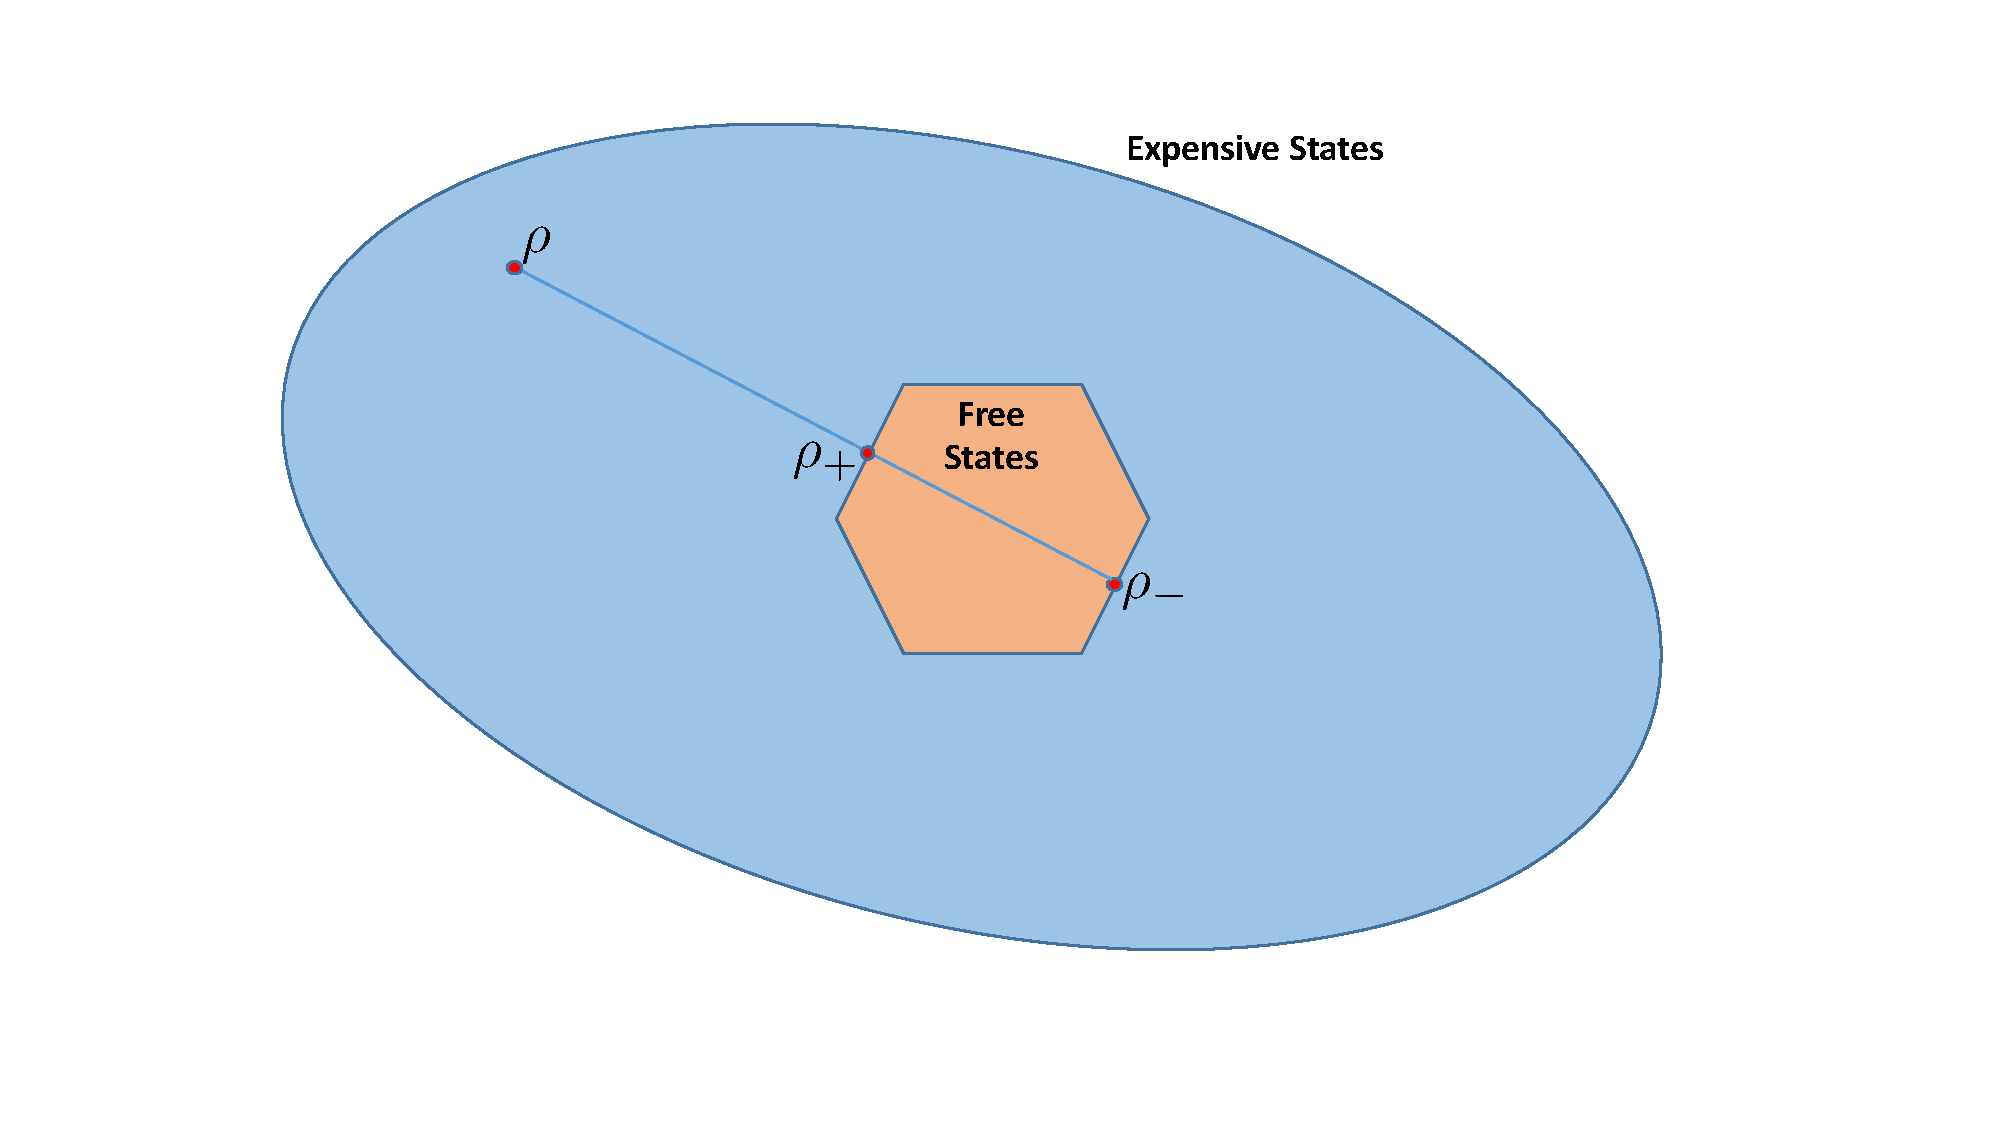
\includegraphics[width=0.7\textwidth]{Figures/Robustness.pdf}
    \caption{Simplified represenation of the robustness measure, showing the definition of the vertices $\rho_{\pm}$ relative to the resource state we wish to quanitity. Depiction inspired by~\cite{Vidal1999,Howard2016}.}
\label{fig:robustshapes}
\end{figure}
This measure can be adapted to different resource states; in particular, we could consider using it to quantify quantum speedup by defining the free resource as the set of efficiently simulabe states, with vertices defined by the stabiliser states. The expensive resource is then the resource states $\ket{R}$ we will use to promote the Clifford circuits to universality~\cite{Howard2016}.\\
The use of Robustness to quantify `magicness' was propsed by Campbell \& Howard~\cite{Howard2016}, motivated by studying contextuality in quantum computing. It is known that for qudits, $d>2$-dimensional quantum states, the onset of Wigner function negativity and contextuality coincide with the definition of magic states. However, qubits display state independent contextuality, and so they sough a measure that would allow them to quantify resource states in qubit and qudit computing. 
\par
It was noted by Campbell \& Howard that the problem of evaluating the Robustness can be converted into a linear programming problem called $\ell_{1}$ minimisation. By defining a matrix $A$ where column $j$ is given by the $j$th vertex of $\mathcal{P}_{free}$. By defining a corresponding column vector $b$ for our resource state, they show that~\cite{Howard2016}
\begin{equation}
    \mathcal{R}(\rho)=\min \norm{x}_{1}\; : Ax=b
\end{equation}
where $\norm{x}_{1}\equiv\sum_{i}\vert x_{i}\vert$.
\par
In their talk, Campbell \& Howard noted that for single magic states $\ket{H}$, evaluating a similar problem called $\ell_{0}$ minimisation gave a related measure 
\begin{equation}
    \mathcal{R}'(\rho)=\min \norm{x}_{0}\; : Ax=b
\end{equation}
that corresponded to the value of the Stabiliser rank decomposition $\chi\left(\ket{H}\right)=2$, where $\norm{x}_{0}\equiv \{\# x_{i} : x_{i}\neq 0\}$, the `sparseness' of the vector $x$~\cite{Howard2016}.\\
This can be understood by considering a the explicit construction of the matrix $A$ and vector $b$ in the case where $\mathcal{P}_{free}$ is defined by the set of stabiliser states. In this case, we can define 
\begin{equation}
    A_{ij}\equiv\braket{i}{\phi_{j}}
\end{equation}
where $\ket{i}$ is the $i$th computational basis state given by the binary representation of the integer $i\in[0,2^{n}-1]$, and $\ket{\phi_{j}}$ is the $j$th Stabiliser state~\cite{Howard2016}. The corresponding definition of $b$ is then
\begin{equation}
    b_{i}\equiv \braket{i}{R}
\end{equation}
where $\ket{R}$ is the resource state we want to analyse.\\
The vector $x$ thus gives the representation of our state in the stabiliser basis, and the sparsest vector should correspond to the optimal stabiliser rank decomposition. 
\par
It is known that the problem of finding the global minimum of the $\ell_{0}$ norm is $\NP$-hard~\cite{ge2011note}. However, as this problem occurs in a signal processing context, fast heurstic algorithms exist. In particular, we implemented a method called `Smoothed $\ell_{0}$' (\texttt{SL0})~\cite{Mohimani2009}. \\
The \texttt{SL0} algorithm works by evaulating an function

\ifstandalone
\bibliography{../MResProject.bib,../ManualEntries.bib}
\fi
\end{document}